\documentclass[convert={density=300,size=1000x500,outext=.png}]{standalone}
\usepackage{tikz}
\usetikzlibrary{arrows}
\usepackage{amsmath}
\usepackage{booktabs}
\usepackage{mathtools}

% arguments are scale and block color
\newcommand{\block}[3]{
    \begin{tikzpicture}[scale=#1]
        \draw[black, sharp corners, fill=#2, line width=1pt] (0,0) rectangle (3, 3);
        \node at (1.5, 1.5) {#3};
    \end{tikzpicture}
}

\begin{document}
\begin{tikzpicture}[scale=0.12]
    \draw[black,line width=2pt] (0,0) rectangle (100, 50);

    \node[draw, rectangle, line width=1pt, align=center] (state) at (15,25) {
        \begin{tabular}{c}
        First-order \\ planning state \\
        \hline
        \\[-5pt]
        \begin{tikzpicture}[scale=0.12]
            \node[align=center] (dummy) at (0,3) {\block{0.12}{red}{}};
            \node[align=center] (dummy) at (0,0) {\block{0.12}{green}{}};
            \node[align=center] (dummy) at (0,6) {\block{0.12}{blue}{}};
            \draw[line width=1] (-3,-1.5) -- (10,-1.5);
        \end{tikzpicture} \\
        $\boldsymbol{+}$ \\
        \\[-5pt]
        $\text{clear}_\text{goal}(\kern-3pt\raisebox{-3pt}{\block{0.12}{red}{}}\kern-3pt)$ \\
        $\text{clear}_\text{goal}(\kern-3pt\raisebox{-3pt}{\block{0.12}{green}{}}\kern-3pt)$ \\
        $\text{clear}_\text{goal}(\kern-3pt\raisebox{-3pt}{\block{0.12}{blue}{}}\kern-3pt)$
    \end{tabular}
    };

    \node[draw, rectangle, line width=1pt, align=center] (feature) at (53,25) {
        \begin{tabular}{c}
            Description logics with \\ planning extensions \\
            \hline
            \rule{0pt}{30pt}
            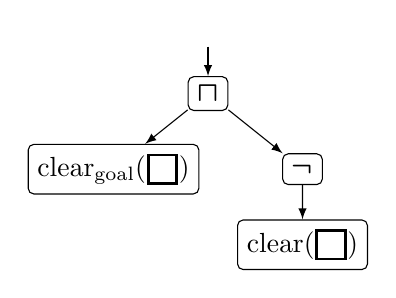
\begin{tikzpicture}[scale=0.12]
                \node[align=center] (dummy) at (0,40) {};
                \node[draw, rectangle, rounded corners=2pt, align=center] (root) at (0,34) {$\boldsymbol{\sqcap}$};
                \node[draw, rectangle, rounded corners=2pt, align=center] (n1) at (-10,26) {$\text{clear}_\text{goal}(\kern-3pt\raisebox{-3pt}{\block{0.12}{white}{}}\kern-3pt)$};
                \node[draw, rectangle, rounded corners=2pt, align=center] (n2) at (10,26) {$\boldsymbol{\neg}$};
                \node[draw, rectangle, rounded corners=2pt, align=center] (n3) at (10,18) {clear(\kern-3pt\raisebox{-3pt}{\block{0.12}{white}{}}\kern-3pt)};

                \draw[-latex] (dummy) -- (root);
                \draw[-latex] (root) -- (n1);
                \draw[-latex] (root) -- (n2);
                \draw[-latex] (n2) -- (n3);
            \end{tikzpicture} \\
            %\hline
            {\tiny ``blocks that are not clear''}
        \end{tabular}};
    \node[draw, rectangle, line width=1pt, align=center] (valuation) at (88,25) {
        \begin{tabular}{c}
            Valuation \\
            \hline
            \\[-5pt]
            $\{\kern-3pt\raisebox{-3pt}{\block{0.12}{red}{}}\kern-3pt,\kern-3pt\raisebox{-3pt}{\block{0.12}{green}{}}\kern-3pt\}$ \\
        \end{tabular}
    };

    \draw[-latex, line width=1pt] (state) -- (feature);
    \draw[-latex, line width=1pt] (feature) -- (valuation);
\end{tikzpicture}
\end{document}